\documentclass[twoside,a4paper,12pt]{uathesis}
\usepackage[percent]{overpic}
\usepackage{algorithm}
\usepackage{algorithmic}

\renewcommand{\algorithmicrequire}{\textbf{Input:}}
\renewcommand{\algorithmicensure}{\textbf{Output:}}

%make fonts searchable
%\usepackage{cmap}
%\input{glyphtounicode}
%\pdfgentounicode=1

\include{preamble}
\DeclareSymbolFont{bbold}{U}{bbold}{m}{n}
\DeclareSymbolFontAlphabet{\mathbbold}{bbold}
\newcommand{\df}{\stackrel{df}{=}}
\newcommand{\dfs}{=_{\scriptstyle{df}}}
\newcommand{\miff}{\mbox{\it iff\/}}
\newcommand{\mi}[1]{\ensuremath{\mathit{#1}}\xspace}
\newcommand{\ignore}[1]{{}}
\newcommand{\Scott}{\ensuremath{\mathbb S}\xspace}
\newcommand{\Real}{\ensuremath{\mathbb R}\xspace}
\newcommand{\Bool}{\ensuremath{\mathbb B}\xspace}
\newcommand{\Nat}{\ensuremath{{\mathbb N}}\xspace}
\newcommand{\cNat}{\ensuremath{{\mathbb N}_{\infty}}\xspace}
\newcommand{\modd}{\ensuremath{\mathrel{\textit{mod}}}\xspace}
\newcommand{\maxd}{\ensuremath{\textit{max}}\xspace}
\newcommand{\mind}{\ensuremath{\textit{min}}\xspace}
\newcommand{\zero}{\ensuremath{\mathbbold{0}}\xspace}
\newcommand{\one}{\ensuremath{\mathbbold{1}}\xspace}

\newcommand{\pr}[1]{{\textsf{\color{red} \small{[#1 -pr-]}}}}
\newcommand{\hp}[1]{{\textsf{\color{red} \small{[#1 -hp-]}}}}
\newcommand{\hw}[1]{{\textsf{\color{red} \small{[#1 -km-]}}}}
\newtheorem{prop}{Proposition}

\usepackage[T1]{fontenc}
\usepackage{lmodern}
\usepackage{amsmath}
%\usepackage{amsfonts}
\usepackage{amsthm}
\usepackage{graphicx}
\usepackage[export]{adjustbox}
\usepackage{url} % format email, hypertext, and path addresses
%\usepackage[figure,linesnumbered,commentsnumbered,shortend,noline]{algorithm2e}
%\usepackage{subfigure}
\usepackage{xspace}

\usepackage{fancyvrb}
%\usepackage{bera} %for bold in verbatim 
%\usepackage{amsmath}
\usepackage{bm}

\usepackage[format=plain,labelfont=up]{caption}
\usepackage{multirow}
\usepackage{xcolor}
\usepackage{colortbl}
%\usepackage[export]{adjustbox} %used to adjust trim image
\usepackage{afterpage}
\usepackage{booktabs} %for tables to use functions such as \toprule
\usepackage{comment}

\usepackage{enumitem} %used to change enum and list spaces and settings

\usepackage{listings}
\lstset{
%     language=C,
    captionpos=b,
    breaklines=true,
%     frame=single,
    basicstyle=\footnotesize,
    numbers=left,
    numberstyle=\bf\scriptsize,
    stepnumber=1,
    numbersep=5pt,
    escapeinside={(*@}{@*)}
%     emph={solution},emphstyle={\color{red}},
%     emph={[2]phOut,oxygenOut,waterOut},emphstyle={[2]\color{blue}},
%     emph={[3]sensors,operatorStop},emphstyle={[3]\color{Green}}
}
\lstdefinelanguage{Esterel}{
    morekeywords={abort, and, await, call, case, combine, constant do, each,
                  else, elsif, emit, end, every, exec, exit, false, function,
                  halt, handle, if, immediate, in, input, inputoutput, loop,
                  mod, module, not, nothing, or,output, pause, positive, pre,
                  present, procedure, relation, repeat, return, run, sensor,
                  signal, suspend, sustain, task, then, tick, timeout, times,
                  trap, true, type, upto, var, watching, weak, when, with
                 },
    sensitive=true,
    morecomment=[l]{\%},
    morestring=[b]",
}

\usepackage{hyperref}
\hypersetup{
    pdfauthor={Keyan Monadjem},
    hidelinks
}
\usepackage{bookmark}

\newbox\subfigbox
\makeatletter
\newenvironment{subfloat}
{\def\caption##1{\gdef\subcapsave{\relax##1}}
  \let\subcapsave\@empty
  \setbox\subfigbox\hbox
  \bgroup}
{\egroup
  \subfigure[\subcapsave]{\box\subfigbox}}
\makeatother

%\newcommand{\comment}[1]{{}}
\newcommand{\dontprintsemicolon}{\DontPrintSemicolon}


%\newtheorem{definition}{Definition}
%\newtheorem{proof}{Proof}
%\newtheorem{theorem}{Theorem}

\newenvironment{abbreviations}{%
    \if@twocolumn
      \@restonecoltrue\onecolumn
    \else
      \@restonecolfalse
    \fi
    \chapter*{List of \abbreviationsname}%
      \@mkboth{\abbreviationsname}%
              {\abbreviationsname}%
  }
  {\newpage\@mkboth{}{}}
\newcommand\abbreviationsname{Abbreviations}

%\begin{filecontents*}{avpedrte.tikz}
%	

\begin{tikzpicture}[>=stealth',shorten >=1pt,auto,node distance=4.5 cm, scale = 1, transform shape]

\tikzstyle{accept} = [draw=blue!75,fill=blue!20]
\tikzstyle{violate} = [draw=red!75,fill=red!20]

\node[initial,state, accepting, accept] (A) {$q_{drive}$};
\node[state, accepting, accept] (B) [right of=A] {$q_{brake}$};
\node[state, violate]         (C) [right of=B]  {$q_v$};

\path[->] 
		(A) edge [loop above]       node [above, xshift=-1em]  
		{
			\scriptsize$\let\scriptstyle\textstyle\substack{\overline{B_H}~\&\\~ \overline{(B_S~\&~(O_{2_P} | O_{5_P}))}, \\ t := 0}$
		} (A)
		
		(A) edge [bend left=45]		node [above]  
		{
			\scriptsize$\let\scriptstyle\textstyle\substack{B_H~|~(B_S~\&\\~(O_{2_P} | O_{5_P})), \\ t := 0}$
		} (B)
	
		(A) edge [bend right=70]	node [above]  
		{
			\scriptsize$\let\scriptstyle\textstyle\substack{\sum\textbackslash \Big((\overline{B_H}~\&~\overline{(B_S~\&~(O_{2_P} | O_{5_P}))})~|\\~B_H~|~(B_S~\&~(O_{2_P} | O_{5_P}))\Big)}$
		} (C)
	
		(B) edge [loop above]		node [above, xshift=2em]  
		{
			\scriptsize$\let\scriptstyle\textstyle\substack{(t < T_{lim}~|~B_H~|~B_S) \\~\&~\overline{A}}$
		} (B)
	
		(B) edge [left]				node [below]  
		{
			\scriptsize$\let\scriptstyle\textstyle\substack{t >= T_{lim}~\& \\ A~\&~\overline{B_H}~\&\\~\overline{(B_S~\&~(O_{2_P} | O_{5_P}))}}$
		} (A)
		
		(B) edge [right]			node [below]  
		{
			\scriptsize$\let\scriptstyle\textstyle\substack{\sum\textbackslash \Big(t < T_{lim}~|~B_H~|~B_S|\\(t >= T_{lim}~\& \\ A~\&~\overline{B_H}~\&\\~\overline{B_S \& (O_{2_P} | O_{5_P})})\Big)}$
		} (C)
	
		(C) edge [loop above]		node [above]  
		{
			\scriptsize$\sum$
		} (C)
		;

\end{tikzpicture}
%\end{filecontents*}
%\begin{filecontents*}{avcarrte.tikz}
%	

\begin{tikzpicture}[>=stealth',shorten >=1pt,auto,node distance=5.5 cm, scale = 1, transform shape]

\tikzstyle{accept} = [draw=blue!75,fill=blue!20]
\tikzstyle{violate} = [draw=red!75,fill=red!20]

\node[initial,state, accepting, accept] (A) {$l_{drive}$};
\node[state, violate]         (C) [right of=A]  {$l_v$};

\path[->] 
		(A) edge [loop above]       node [above, xshift=-1em]  
		{
			\scriptsize$\let\scriptstyle\textstyle\substack{B_S~\&~(O_{2_C}~|~O_{5_C})~\&\\~(S~>~O_{2_V}~|~S~>~O_{5_V})~|\\~A~\&~O_{4_C}~\&~S~<~O_{4_V}}$
		} (A)
	
		(A) edge [right]	node [above]  
		{
			\scriptsize$\let\scriptstyle\textstyle\substack{\sum\textbackslash \Big(B_S~\&~(O_{2_C}~|~O_{5_C})~\&\\~(S~>~O_{2_V}~|~S~>~O_{5_V})~|\\~A~\&~O_{4_C}~\&~S~<~O_{4_V}\Big)}$
		} (C)
	
		(C) edge [loop above]		node [above]  
		{
			\scriptsize$\sum$
		} (C)
		;

\end{tikzpicture}
%\end{filecontents*}
%\begin{filecontents*}{avdriverte.tikz}
%	

\begin{tikzpicture}[>=stealth',shorten >=1pt,auto,node distance=5.5 cm, scale = 1, transform shape]

\tikzstyle{accept} = [draw=blue!75,fill=blue!20]
\tikzstyle{violate} = [draw=red!75,fill=red!20]

\node[initial,state, accepting, accept] (A) {$q_{drive}$};
\node[state, violate]         (C) [right of=A]  {$q_v$};

\path[->] 
(A) edge [loop above]       node [above, xshift=-1em]  
{
	\scriptsize$\let\scriptstyle\textstyle\substack{A~\&~S~<=~100~|\\~(H_B~|~S_B)~\&~S~>=~0}$
} (A)

(A) edge [right]	node [above]  
{
	\scriptsize$\let\scriptstyle\textstyle\substack{\sum\textbackslash \Big(A~\&~S~<=~100~|\\~(H_B~|~S_B)~\&~S~>=~0\Big)}$
} (C)

(C) edge [loop above]		node [above]  
{
	\scriptsize$\sum$
} (C)
;

\end{tikzpicture}
%\end{filecontents*}
%\begin{filecontents*}{avcnnrte.tikz}
%	\input{Content/fig/av-cnn-rte.tex}
%\end{filecontents*}

\begin{filecontents*}{avgraph.tikz}
	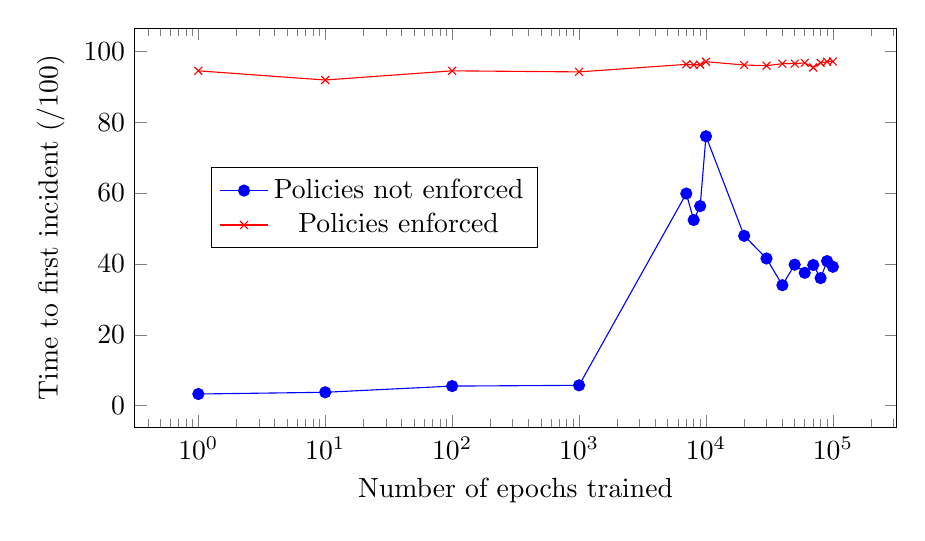
\begin{tikzpicture}
\begin{semilogxaxis}[
xlabel={Number of epochs trained},
ylabel={Time to first incident (/100)},
x=0.7cm,
y=0.45mm, 
legend style={at={(0.1,0.55)},anchor=west}]

\addplot[color=blue,mark=*] coordinates {
	(0, 3.24)
	(1, 3.29)
	(10, 3.78)
	(100, 5.53)
	(1000, 5.74)
	(7000, 59.87)
	(8000, 52.39)
	(9000, 56.33)
	(10000, 76.03)
	(20000, 47.94)
	(30000, 41.54)
	(40000, 34)
	(50000, 39.8)
	(60000, 37.5)
	(70000, 39.7)
	(80000, 36)
	(90000, 40.8)
	(100000, 39.2)
};

\addplot[color=red,mark=x] coordinates {
	(0, 93.2)
	(1, 94.5)
	(10, 91.91)
	(100, 94.5)
	(1000, 94.2)
	(7000, 96.33)
	(8000, 96.21)
	(9000, 96.24)
	(10000, 97.07)
	(20000, 96.15)
	(30000, 95.94)
	(40000, 96.52)
	(50000, 96.53)
	(60000, 96.74)
	(70000, 95.44)
	(80000, 96.75)
	(90000, 97.09)
	(100000, 97.14)
};

\legend{Policies not enforced, Policies enforced}
\end{semilogxaxis}%
\end{tikzpicture}%
\end{filecontents*}

\begin{document}

\title{Safe Synchronous Artificial Neural Networks}
\author{Keyan Themba Monadjem}
\department{Electrical \& Computer Engineering}
\submitdate{February 2019}
\supervisor[Dr. Partha S. Roop]

%create the title page
\maketitle

%%%%%%%%%%%%% First section %%%%%%%%%%%%%%%
\frontmatter
\bookmark[page=3]{Abstract}
\include{Abstract}

\bookmark[page=5]{Acknowledgements}
\include{Acknowledgements}

%create table of contents
\bookmark[page=7]{Contents} % Sets a PDF bookmark for the contents page
\tableofcontents

\bookmark[page=11]{List of Figures}
\listoffigures

\bookmark[page=15]{List of Tables}
\listoftables

%\cleardoublepage
%\phantomsection
%\addcontentsline{toc}{chapter}{List of Abbreviations}
%\input{abbreviations}

%%%%%%%%%%%% Body of the Thesis %%%%%%%%%%%
\mainmatter

\acrodef{WCRT}{Worst Case Reaction Time}
\acrodef{WCET}{Worst Case Execution Time}
\acrodef{SOT}{Start Of Tick}
\acrodef{EOT}{End Of Tick}
\acrodef{CPS}{Cyber-Physical System}
\acrodef{AI}{Artificial Intelligence}

\acrodef{ESS}{Energy Storage System}
\acrodef{SoC}{State of Charge}
\acrodef{MBD}{Model-Based Design}
\acrodef{FPGA}Field-Programmable Gate Array}

\acrodef{CFG}{Control Flow Graph}
\acrodef{TCFG}{Timed Control Flow Graph}
\acrodef{TCCFG}{Timed Concurrent Control Flow Graph}
\acrodef{TCA}{Tick Cost Automata}

\acrodef{NN}{Neural Network}
\acrodef{DNN}{Deep Neural Network}
\acrodef{SNN}{Synchronous Neural Network}
\acrodef{CNN}{Convolutional Neural Network}
\acrodef{SANN}{Synchronous Artificial Neural Network}
\acrodef{SNN}{Synchronous Neural Network}
\acrodef{SSNN}{Safe Synchronous Neural Network}
\acrodef{ANN}{Artificial Neural Network}
\acrodef{RNN}{Recurrent Neural Network}
\acrodef{MLP}{Multi-layer Perceptron}
\acrodef{MNN}{Meta Neural Network}
\acrodef{MNN2C}{Meta Neural Network to C}

\acrodef{AV}{Autonomous Vehicle}
\acrodef{LiDAR}{Light Detection and Ranging}

\acrodef{VOC}{Visual Object Classes}
\acrodef{GTSRB}{German Traffic Sign Recognition Benchmark}

\acrodef{VDTA}{Valued Discrete Timed Automata}
\acrodef{DTA}{Discrete Timed Automata}
\acrodef{RE}{Runtime Enforcement}
\acrodef{RA}{Runtime Assurance}

\chapter{Introduction}

\section{Cyber-Physical Systems}
Introduce the concept of safety critical, CPS. What makes a system safety critical?

\section{Artificial Neural Networks}
Introduce AI, more specifically ANNs. What they can do?

\section{Contribution}
Creating methods of implementing ANNs in safety critical systems using synchronous semantics.

\section{Thesis Structure}
Chapter 2 gives a basic understanding of the concepts required to understand this research towards safe \acp{ANN} for \ac{CPS}.

Chapter 3 introduces the concept of \acfp{SANN} and their timing properties.
Formal definitions of \acp{SANN} and their related components are provided in this chapter.
Furthermore, the combinations of these \acp{SANN} and the usefulness of such in \ac{CPS} is discussed.
A new compiler to create these \acp{SANN} from Python code is also introduced.

Chapter 4 introduces the concept of \acf{RE} in combination with \acp{SANN}. 
This chapter also provides formal definitions for the combination of \acp{SANN} and \ac{RE} by expanding the definitions introduced in Chapter 3.
An \acf{AV} case study is made for this chapter.

Chapter 5 provides two different methods, used in tandem, to increase the safety of systems with complex inputs, such as object detection for \acp{AV}.
The first method is the use of \acp{MNN} to increase the classification accuracy of \acp{SANN}.
The second expands on Chapter 5, and introduces the use of \acf{RV} to increase the safety of system where \ac{RE} is impossible.
Results are presented using another \ac{AV} system case study.



\chapter{Background}

\section{Artificial Neural Networks}
\subsection{Machine Learning}
\acp{ANN} were originally proposed to mimic the functioning of  biological neural networks~\cite{kohonen1988introduction}, which produce recurrent spatio temporal patterns~\cite{rolston2007precisely}. 
Similar timed activity of neurons in the cerebellum has been reported in~\cite{bullock1994neural, moore1989adaptively}. 
A number of types of \ac{NN} which mimic their biological counterparts exist, varying in complexity and accuracy, including the \ac{SNN}~\cite{izhikevich2003spiking,maass1997spiking}, which was designed to model the brain and has been demonstrated to be periodic and run with discrete time intervals when implemented in software. 

\subsection{Structure of an Artificial Neural Network}
Most \acp{ANN} do not feature such complex models like those of spiking neural networks, as they are more difficult to use, implement, and train. 
Instead, they rely on simpler networks, which can be considered as \emph{un-timed non-linear} functions, where the outputs change relative to the inputs, but the timing of the change is not precisely defined. 
An example of such a network is provided in Figure~\ref{fig:mlp-ann}, which is using neurons defined in Figure~\ref{fig:artificial-neuron}. 
This is a type of \ac{NN} known as an \acf{MLP}~\cite{yegnanarayana1994artificial}.

Specialised neural networks, called \acfp{RNN}~\cite{medsker2001recurrent}, were introduced to classify temporal sequences. 
These operate in a step by step manner, where the operation in the current time step relies on the context from some previous step. Thus, \acp{RNN} may be viewed as a periodic networks, whosemperiod is one. 
However, the use of such networks in \ac{CPS} is yet to be thoroughly investigated. 
Moreover, \acp{RNN} and their compositions are not formalised especially from the point of view of designing timed AI systems used in \ac{CPS}.  

\begin{figure}
	\centering
	\scalebox{0.8}{\input{fig/mlp-ann.tex}}
	\caption{Example \ac{MLP} \ac{ANN}.	\label{fig:mlp-ann}}
\end{figure}
\begin{figure}
	\centering
	\scalebox{0.8}{\input{fig/neuron.tex}}
	\caption{A model of an artificial neuron. \label{fig:artificial-neuron}}
\end{figure}

\acp{ANN} are being increasingly used as controllers in \acp{CPS} due to their ability to learn data relationships in ways that are difficult to replicate~\cite{ANNSafety2007}. 
\acp{ANN} can deal with novel inputs to the system and are able to outperform other forms of \ac{AI} at computational efficiency, pattern recognition, function approximation and image identification~\cite{AIComp2016, AIComp2017}. 
However, it can be very difficult to ensure the safety of a system involving \acp{ANN}~\cite{ANNSafety2007, ANNSafety2018}.

\subsection{Safety of Artificial Neural Networks}
In order for an \ac{ANN} to be used in any capacity within a \acp{SCS}, it should undergo rigorous and thorough validation, verification, and testing procedures to ensure that they it is sufficiently safe for its target system~\cite{scann, ANNSafetyLifecycle2003}. 

While considerable research effort is starting in the direction of formal verification of \ac{AI}-based \ac{CPS}~\cite{seshia2016towards, russell2015}, the issue of timing verification has received scant attention. 
Like the challenges involving functional verification, timing verification of AI-based  \ac{CPS} poses considerable challenges due to: (1) real-time \ac{AI} systems could involve many concurrent and interacting \ac{AI} modules, which need deterministic composition for safety; (2) \ac{AI} modules are usually developed as untimed systems and the reactive nature of AI algorithms used in CPS are not carefully studied; and (3) \acf{WCET} analysis~\cite{wilhelm2008worst} of \ac{AI}-based \ac{CPS} has received scant attention.

Definitions for this safety vary, but Kurd et. al.~\cite{EstSafeCriteria2003} provide a generalisation: safe \acp{ANN} can be defined as those that:
\begin{itemize}
	\item tolerate faults and inconsistencies in their inputs,
	\item do not create hazardous outputs,
	\item behave in a predictable and repeatable manner,
	\item and are trained on clean, reliable data. 
\end{itemize}
%These properties are essential for an \ac{ANN} to run in any \ac{SCS}. 

To achieve these properties, there exist safety measures such as risk management systems that span the entire development process of the \ac{ANN}~\cite{ANNDevModel1999} and standards with which \acp{ANN} can be certified before they are used in \acp{SCS}~\cite{SCANNStandard}. 
These techniques are primarily \textit{proactive} in nature, producing \acp{ANN} that are classified as \textit{safe enough} for their role. 

However, as \acp{ANN} become larger and more full-featured, they  become harder to statically analyse.
Problematic situations can arise when an \ac{ANN} exhibits unexpected behaviour that the system is unable to safely respond to, and in \acp{SCS} these situations can be life threatening.







\section{Timing Analysis of Cyber-Physical Systems}
\subsection{Worst Case Execution Time}
Explain what WCET is in safety critical systems. Why is it important for deadlines to be met and how does this relate to WCET?

\subsection{Worst Case Reaction Time}
WCRT vs WCET. Throughput vs Time.

\subsection{Timing Techniques}
What timing techniques exist for synchronous and asynchronous systems? Which of these are relevant to our work?

\subsection{Patmos Time Predictable Processor}
Brief description of Patmos and why we use it.








\section{Static Verification of Artificial Neural Networks}
This section looks into ANN verification methods and why they are good/bad.

\subsection{The Problem of Artificial Neural Network Verification}
ANN verification is an issue. Why?

\subsection{Existing Techniques for Verifying ANNs}
Rundown of existing techniques of ANN verification.

\subsection{Limitations of Artificial Neural Network Verification}
Describe where verification is limited and why.
Where can it do better?





\section{Synchronous Languages}
\subsection{Synchronous Semantics}
Briefly explain synchronous semantics: what is synchronous programming and how does it work?

\subsection{Safety of Synchronous Languages}
What guarantees does synchronous programming provide?
Determinism
Causality
Easy to formalise
Etc

\subsection{Timing Correctness}
Time predictability.

\subsection{Functional Correctness}
Runtime Enforcement






\section{Run-time Enforcement}
\subsection{Run-time Assurance}
What is RA and why is it useful? Formally defined.

\subsection{Run-time Monitoring}
How does this relate and improve on RA?

\subsection{Run-time Enforcement}
Benefits? Synchronous vs asynchronous systems. 

\subsection{Safety (Timed) Automata}
These are used in our run-time enforcement techniques. Discuss these and how they work.





\section{Summary}
Summary of above.

\chapter{Synchronous Neural Networks}

%\section{Esterel, Synchronous Programming Language}
\subsection{Fundamentals of Esterel}
Briefly describe the synchronous keywords used in Esterel and how they make it a synchronous language.

\subsection{Compiling Esterel}
Explain the process behind creating code in Esterel, compiling it to C and then using the C as part of a program.


\section{Synchronous Neural Networks}
\subsection{Fundamentals of Artificial Neural Networks}
Explain what is needed in an ANN library.

\subsection{Architecture of Synchronous Neural Networks}
Describe how SNNs run and how they work as an ANN library.

\subsection{Formalalisation of Synchronous Neural Networks}
This subsection provides a formal definition for feed forward SNNs

\subsection{Implementation of Synchronous Neural Networks}
Describe how to use the SNN library. Describe both the C and Esterel aspects of SNNs.

\section{Timing Analysis of \acfp{SNN}}
\label{sec:wcrt}

Time in a synchronous program progresses in logical discrete instants called \emph{ticks}. 
In each tick, the environment is first sampled, then computation takes places, and finally the results are emitted.
In order for safety-critical \ac{CPS}, such as our \texttt{AI-BRO}, to be verified, we need to ensure that the time taken for the execution of any given tick is less than their environmental deadlines.
This necessitates the computation of the worst-case tick length via static timing analysis --- also known as \acf{WCRT} analysis~\cite{roop2009tight}.

\ac{WCRT} analysis needs two things: (1) an architectural model of the
underlying processor architecture; and (2) a \acf{CFG}~\cite{wilhelm2008worst}  representation of
binary program execution over the architectural model. The analysis
process then computes the longest path through the \ac{CFG}.
%For any program, static timing analysis involves first the derivation of a \acf{CFG}~\cite{wilhelm2008worst} which captures the possible execution traces.
%Then, the \ac{CFG} must be annotated with the time taken to execute each node, so that a worst-case path can be derived.
While general purpose programs can feature complications which make this process difficult, Esterel is ideally suited to derivation of \acp{CFG} due to inherent features:  (1) all loops in Esterel are bounded, as there is a need for at least one \texttt{pause} statement
within every loop; and (2) compilers ``compile-away'' the logical
concurrency to produce sequential code. However, as can be seen in
Listing~\ref{lst:ai-bro}, 
Esterel programs can also invoke arbitrary C-functions, which may use
features such as function pointers, unbounded loops, and external interrupts. 
To this end, we provide a set of guidelines and \ac{ANN}
implementation libraries in C,
which restrict these features to make each C function call time
analysable. 

%\subsection{Guidelines}
In this paper, we are using the open-source Platin
tool~\cite{compiler:platin:kps15} for \ac{WCRT}
analysis. Consequently, we have to consider some tool-specific
restrictions to avoid the use of generic features in C that are not
suitable for static analysis, such as system calls, function pointers, interrupt-driven flow, or unbounded loops~\cite{RTOSWCET}.
Hence, the restrictions considered in this paper are: (1) all neural
network functions are coded as bounded \texttt{for} loops; (2) all
memory is statically allocated; (3) variable-length array iterator
functions are coded using preprocessor macros; and (4) the final binary is executed `bare-metal', requiring no
RTOS or OS support, thus avoiding scheduling dependencies
that may be difficult to statically analyse.
\ignore{
	\begin{itemize}
		\item All neural network functions are coded as bounded \texttt{for} loops.
		\item All memory is statically allocated.
		\item Variable-length array iterator functions are coded using preprocessor macros.
		\item The final binary is executed `bare-metal', requiring no
		RTOS or OS support, thus avoiding scheduling dependencies
		that may be difficult to statically analyse.
	\end{itemize}
}

Annotating a \ac{CFG} with execution times is no simple task for many architectures.
Enhancements such as out-of-order execution, multi-level caches, and deep pipelines can all cause complications when considering the time taken to execute program code.
For instance, in~\cite{AirplaneWcet}, Ferdinand et. al. demonstrate the difficulties of determining the worst-case time in arguably simple avionics code running on a Motorola ColdFire 5307.
To avoid these complications, we rely on the Patmos~\cite{patmos:ppes2011} architecture, which is a simple RISC pipeline optimised for static timing analysis. 
Here, caches have simple replacement policies, and it also has a time-predictable memory hierarchy.
It relies on an adaptation of the LLVM compiler that targets the Patmos instruction set.
This simplifies the annotation of the nodes of the \ac{CFG} with
timing costs, thus allowing for a straightforward static analysis of any
\ac{SNN}. Consequently, this work is restricted to the single-core
Patmos architecture and does not examine execution of \acp{SNN} on
other platform types, such as Intel processors and GPUs.
%\changed{Consequently, this work is restricted to the single-core Patmos architecture and does not examine execution of \acp{SNN} on other platform types, such as Intel processors or GPUs}.

%The expense of this is program size, and designers can expect slightly increased program memory usage as a result. 

%When it comes to the annotation of these nodes with their execution times, architectural considerations must be taken into account, for instance memory access times and pipelined execution of instructions.


%\subsection{Patmos}


%We then use the open-source academic timing analysis tool called Platin~\cite{compiler:platin:kps15}, to derive our execution times.


\ignore{
	\begin{example}
		Consider the case of our AI-BRO example in Listing~\ref{lst:ai-bro}. 
		We can express this Esterel program using the \ac{CFG} presented in Figure~\ref{fig:cfg-aibro}.
		\begin{figure}
			\centering
			\begin{tikzpicture}[->,>=stealth',shorten >=1pt,auto,
	node distance=2.5cm,
	semithick,scale=0.8, transform shape,scale=0.6, font=\huge]
	
	\tikzstyle{every state}=[rectangle,
	minimum height = 1cm, text width=3.5cm, text centered, 
	fill=blue!20,draw=none,text=black, draw,line width=0.3mm, font=\LARGE]
	
	%start state
	\node[state]
	(init) 
	{$f$: \\init, \textit{fork}}; 
	
	\node[state]
	(awaitA) [below of=init] 
	{$a_1$: \\await \texttt{A}};
	
	\node[state]
	(frontA) [below of=awaitA] 
	{$a_2$: \\frontSensors()};
	
	\node[state]
	(awaitB) [below of=frontA]
	{$b_1$: \\await \texttt{B}};
	
	\node[state]
	(sideB) [below of=awaitB]
	{$b_2$: \\sideSensors()};
	
	\node[state]
	(awaitJoin) [below of=sideB] 
	{$j$: \\ \textit{await join}};
	
	\node[state]
	(decisionC) [below of=awaitJoin] 
	{$c$: \\runDecision()};
	%\node[draw=none]
	%(inv) [below of=init]
	%{};
	
	%\node[draw=none]
	%(inv2) [below of=inv]
	%{};
		
	

	
	\path[->] (init) edge (awaitA);
	\path[->] (awaitA) edge (frontA);
	\path[->] (frontA) edge (awaitB);
	\path[->] (awaitB) edge (sideB);
	\path[->] (sideB) edge (awaitJoin);
	\path[->] (awaitJoin) edge (decisionC);
	
	\draw[->] (decisionC.south) 
		|- ($(decisionC.south) + (0, -1cm)$) 
		-| ($(decisionC.east) + (2.5cm, 0)$) 
		|- ($(init.east) + (0, 1.5cm)$) 
		-| (init.north);
		
	\draw[->] (awaitA.west) 
		-| ($(awaitA.west) + (-1cm, 0)$)
		|- ($(awaitB.west) + (-1cm, 0)$)
		%|- ($(awaitA.160) + (0, 0.75cm)$) 
		|- (awaitB.west);
		
	\draw[->] (awaitA.west) 
		-| ($(awaitA.west) + (-1cm, 0)$)
		|- ($(awaitB.west) + (-1cm, 0)$)
		%|- ($(awaitA.160) + (0, 0.75cm)$) 
		|- (awaitJoin.west);
		
	\draw[->] (awaitB.east) 
		|- ($(awaitB.east) + (2.5cm, 0)$);
		
	\draw[->] (awaitJoin.east) 
	|- ($(awaitJoin.east) + (2.5cm, 0)$);
	
	%\draw[->] (decisionC.south) 
	%	|- ($(decisionC.south) + (0, -1cm)$) 
	%	-| ($(decisionC.east) + (4.5cm, 0)$) 
	%	|- ($(init.east) + (0, 1.5cm)$) 
	%	-| (init.north);
	
	%\draw[->] (awaitA.200) 
	%	|- ($(awaitA.200) + (0, -0.75cm)$) 
	%	-| ($(awaitA.200) + (-2cm, 0)$)
	%	|- ($(awaitA.160) + (0, 0.75cm)$) 
	%	-| (awaitA.160);
		
	%\draw[->] (awaitB.340) 
	%|- ($(awaitB.340) + (0, -0.75cm)$) 
	%-| ($(awaitB.340) + (2cm, 0)$)
	%|- ($(awaitB.20) + (0, 0.75cm)$) 
	%-| (awaitB.20);
	
	%\draw[->] (awaitJoin.195) 
	%|- ($(awaitJoin.195) + (0, -0.75cm)$) 
	%-| ($(awaitJoin.195) + (-1.5cm, 0)$)
	%|- ($(awaitJoin.165) + (0, 0.75cm)$) 
	%-| (awaitJoin.165);
	
	
\end{tikzpicture}

			\caption{Single-thread AI-BRO \ac{CFG}}
			\label{fig:cfg-aibro}
		\end{figure}
	\end{example} \pr{This figure is somewhat non-standard. There are no
		conditional nodes. I suggest you examine the syntax of CFGs
		presented in WCET papers and follow these.}
}

%Fortunately, it is straightforward to convert the synchronous C code generated by Esterel into its equivalent control flow graph.
%Then, as long as the external C function calls that it will call are also predictable, and if the code is run on a time-predictable architecture such as Patmos~\cite{patmos:ppes2011}, the code can be %converted into an equivalent \ac{TCFG}.


%This section discusses the WCRT analysis of SNNs.
%Introduce the WCET problem and then introduce WCRT.
%Intermediate format, timing model, the PATMOS core.
%Coding guidelines for time analysable code. Steps to improve the 
%WCRT. These can be the various subsections.


%When considering normal C code, such as in our external function calls, it can be extremely difficult to construct \ac{CFG}.
%This is because it can be difficult to statically an
%Constructing a \ac{CFG} for a normal general purpose program can be very difficult, especially if it relies on complex software constructs such as system calls, function pointers, interrupts, or unbounded loops.
%This is because the construction of the \ac{CFG} becomes extremely difficult in the face of large branching potentials or unknown jump destinations.


\subsection{\ac{WCRT} algebra}
\label{sec:wcrt-algebra}

Though Esterel is amenable to timing analysis, it still suffers from state space explosion when considering large programs. 
Analysing large sequential code generated from Esterel compilers that ignore \emph{infeasible state space} 
produce large overestimates. \ac{WCRT} algebra, presented in \cite{wang2017timing}, presents a solution to this problem: large synchronous programs can be expressed as 
networks of simpler \ac{TCA}, which have equivalent timing properties to their \ac{TCFG} counterparts. Considering this, we
seek to use this framework to develop a compositional timing semantics of \acp{SNN} and their compositions.

We consider a discrete max-plus structure over
natural numbers $(\Nat_{\infty}, \oplus, \odot, \zero, \one)$ where:
\begin{itemize}
	\item $\Nat_{\infty} \dfs \Nat \cup \{ -\infty, +\infty \}$
	\item  $\oplus$ and $\odot$ are commutative and associate operators that 
	denote the maximum and addition respectively on $\Nat_{\infty}$. 
	\item Neutral elements are $\zero \dfs -\infty$ and $\one \dfs 0$,
	respectively, i.e., $x \oplus \zero = x$ and $x \odot \one = x$. 
\end{itemize}

In particular, $-\infty \odot +\infty = -\infty$. Addition
$\odot$ distributes over max $\oplus$, i.e.,
$x \odot \left(y \oplus z\right) = x + \maxd\left(y, z\right) = \maxd\left(x + y, x + z\right) =
\left(x \odot y\right) \oplus \left(x \odot z\right)$. However, $\oplus$ does not distribute
over $\odot$, for instance, $9 \oplus \left(5 \odot 7\right) = \maxd\left(9, 5 + 7\right) = 12$
while $\left(9 \oplus 5\right) \odot \left(9 \oplus 7\right) = \maxd\left(9, 5\right) + \maxd\left(9, 7\right) = 18$.
This induces on $\Nat_{\infty}$ a (commutative, idempotent) semi-ring.
We denote $\mathcal{W}$ as the set of formulae in this algebra.

We use an automaton called \ac{TCA} to capture the timing behaviour of any \ac{SNN}.
These are mono-cyclic automata, where every state of the automaton is labelled by a
WCRT formula that associates the state with its worst case timing cost.
We start by defining \ac{TCA} using Definition~\ref{def:tca}
%---------------------------------

\begin{definition}
	A \emph{mono-cyclic tick cost automaton}, here after referred to as tick cost automaton (\ac{TCA}) 
	is %a tuple 
	$M = \langle Q, q_0, \rightarrow, \mathcal{W}, L
	\rangle$, where $Q$ is a finite set of \emph{states} with a
	distinguished \emph{entry} state $q_0 \in Q$ and $L: Q \rightarrow \mathcal{W}$ is
	a labeling function that labels every state with its associated timing cost by a formula in $\mathcal{W}$.
	The \emph{transition relation}
	${\rightarrow} \subseteq Q \times Q$ satisfying the following:
	
	\begin{enumerate}
		\item From any state $q_i \in Q$ there is at most one transition to a successor state $q_j \in Q$.
		\item The transitions are such that they form a mono-cycle that starts in $q_0$ and and ends in a 
		transition from some state $q_{n-1} \rightarrow q_0$, resulting in a
		cycle of length $n \in \Nat_{>0}$.
		\item A \ac{TCA} whose cycle length is $1$ is termed
		\emph{mono-periodic}, while those with cycle length $>1$ are called
		\emph{multi-periodic}.
		\item The \emph{reaction time} of a \ac{TCA} is its tick-length, which is
		always fixed to its \ac{WCRT}. 
		\item The \emph{response time} of a \ac{TCA} is the time taken for the
		corresponding \ac{SNN} to produce the outputs given inputs. 
		The response time of a TCA is given by the formula $n \times WCRT$,
		where $n$ is the cycle length.
		%\item The above conditions ensure that a \ac{TCA} is a mono-cyclic automaton.
	\end{enumerate}
	\label{def:tca}
\end{definition}

%---------------------------------
\ignore{
	\pr{Hammond: I have defined both reaction and response time of a
		TCA. We should use these      n our benchmarks, if possible.}
	\begin{example}
		$15 \oplus \left(5 \odot 10\right) = 15$, and $\left(15 \oplus 5\right) \odot \left(15 \oplus 10\right) = 30$.
	\end{example}
	
	\begin{example}
		Consider the program in Listing~\ref{lst:ai-bro}. 
		This had two concurrent threads, which are compiled away to produce sequential code.
		We can express this network's \ac{WCRT} as \\
		$WCRT = \left( a_{await} \odot a_{run} \odot b_{await} \odot b_{run} \odot c_{awaitJoin} \odot c_{run} \odot c_{emit} \right)$, as this is the longest potential path through the system (if we receive both \texttt{A} and \texttt{B} in the same tick).
	\end{example} \pr{Hammond -- since the figure is removed, this formula
		doesn't make any sense now. Please check.}}
%$x \oplus y =$ $MAX(x,y)$ 
%$x \odot y =$ $x + y$ 
\section{Case study: \acf{AV} braking}
\label{sec:case}

%The research and development of safe \acp{AV} is a competitive topic. 
\ac{AV} are safety critical \acfp{CPS} as any faults in their operation can lead to accidents resulting in injuries or fatalities. 
%What constitutes a safe \ac{AV} and the design of these systems is a highly controversial topic. 
Unfortunately, such faults have already occurred.
For instance, both Tesla and Uber have had autonomous vehicle accidents~\cite{stewart_2018,coldewey_2018}.

It is difficult to build complete models of these scenarios, as \ac{AV} companies tend to produce or customise their own vehicles with their own proprietary hardware and software.
Nevertheless, in this paper, we use these unfortunate incidents as inspiration for a case study for this paper, where we examine one aspect of \ac{AV} control: the braking mechanism.
%, designed differently to each other competitor, and each company has its own, unique issues with the safety of these systems.
%Each time an incident with an \ac{AV} system occurs, it hits the news headlines.
%Recently, Tesla and Uber vehicles' fatal accidents have been making news.

%In this case study we 
%However, the \ac{AV} system in this paper was designed with only the braking aspect of \ac{AV} systems in mind. 
Here, we integrate a sensor package consisting of five cameras and a \ac{LiDAR} sensor. 
Each of the five cameras feeds into an \ac{ANN} ensemble~\cite{Maqsood2004} of CNNs, using the Darknet library~\cite{darknet13}.
These ensembles classify their input image and provide a confidence level for the classified image, before passing this information to the controller.
The controller \ac{ANN} is a \ac{MLP}, and decides the best course of action given the environment and the status of the vehicle itself. 
It then outputs controls to the vehicles actuators, which in our case are represented by an accelerator and a brake.
%Finally, the controller outputs are sent back to the vehicle, where the actuators are then updated accordingly.
%Here, the actuators for this system are the accelerator, which increases the speed of the vehicle; and the brakes, which slow down the vehicle.
A diagram of the \ac{AV} used in this system is shown in Figure~\ref{fig:av}. \todo{Consider adding a figure showing the NN layout}

\begin{figure}[t]
	\centering
	\includegraphics[width=\linewidth]{Content/fig/AV.pdf}
	\caption{Diagram showing the sensor layout for the \ac{AV}. \label{fig:av}}
\end{figure}

The controller \ac{MLP} takes seventeen different inputs. 
Two inputs correspond to the current speed of the vehicle ($S$) and the speed of the vehicle one tick in the past ($P$). 
The other fifteen inputs are broken into three boolean inputs for each camera's detected object ($O_1$ - $O_5$): the type of object seen in that camera ($N$: nothing, $P$: pedestrian, $C$: car or $U$: unknown), the speed of the object ($V$) and the direction of the object ($D$).
E.g. a car far in-front of the \ac{AV} would be represented by $O_5$ as $O_{5_C}$, and its speed and direction by $O_{5_V}$ and $O_{5_D}$ respectively.
Depending on these inputs, the controller outputs three values  $A$: accelerate, $B_S$ soft brake, or $B_H$: hard brake.
These outputs can each be between 0 and 1.
If any of the values exceed 0.1, the highest valued action is chosen, otherwise the vehicle takes no action, i.e. it will continue at current speed (which could be zero).

Due to this design of this system, it is possible for the vehicle to behave badly in various ways. 
These include not driving at all, speeding, unnecessarily slamming the brakes, hitting other vehicles on the road and hitting pedestrians both on and off the road.
%All of these scenarios can result in fatalities, thus classifying this system as a \ac{SCS}.
To have a system that is safe, policies need to be enforced that monitor the system's inputs and outputs and ensure that none of the above scenarios take place under any circumstances.
%This system is designed for two purposes: (1) to conceptualize \acp{SNN} and show their architecture; and (2) to show the efficacy of these \acp{SNN}.

\subsection{\acf{RE}}
%% TALK ABOUT RA AND RE
%\todo{Move this to lit review?}
% Runtime assurance
\ac{RA} is the ability to to ensure that a system operates safely, even when the system contains components that are not sufficiently reliable or verified~\cite{rta-cps}. 
Thus, \ac{RA} can be used to bound unpredictable or unsafe behaviour in a target system. 
\ac{RA} has been used as a reliability and fail-safe tool for some time, for instance in \acp{OS}, intrusion detection, overcurrent breakers and flight controllers. 
A system that uses \ac{RA} shifts the burden of testing and analysing system parameters from comprehensive off-line verification methods, to a simpler assurance mechanism~\cite{rta-cps}. 
%This technique has already been suggested for the certification of modern \acp{CPS}. 

% Runtime enforcement
\ac{RE} is a subset of \ac{RA} that focuses on formal semantics.
Traditionally, \ac{RE} is developed for reactive systems, where it is able to block, delay, modify and/or re-order events in a system. 
Processes that are deemed unsafe can be monitored by an enforcer at runtime to ensure that they obey desired policies and remain in a safe state at all times~\cite{theoryRE}. 
\ac{SA} formally express run-time properties that can be monitored in one direction only (e.g. outputs only)~\cite{enfsafepol}. 
Edit automata are a type of \ac{SA} that can edit, suppress or insert events~\cite{editautomata}. 
Safety Automata (or \ac{DTA}) have been proposed that can edit \textit{bi-directional} events at runtime~\cite{recps}. 
They were designed for reactive \acp{CPS} demonstrated in a pacemaker environment~\cite{recps}. 
%This paper looks at the use of bi-directional \ac{RE} to enforce safety policies defined as Safety Automata in reactive, autonomous environments. 

\ac{SRE} allows for easier formal reasoning over the possible runtime behaviour of the \acp{ANN} internal to the system, thus no longer requiring difficult static analysis.
\ac{SRE} can apply a set of policies on the inputs and outputs of the system to ensure it follows a set of given constraints. % \acp{SANN} to ensure that the policies are never violated. 
These policies can also feature timing information to guarantee timing deadlines for real-time systems.
A well designed policy can thus ensure that the system never exhibits unsafe events --- therefore keeping the system's inputs and outputs \textit{safe}~\cite{EstSafeCriteria2003}. 

However, these \ac{RE} models look at the enforced system as a black box. 
For the purpose of \ac{RE} of an \ac{SANN} and its timed properties, the \ac{SANN} needs to be viewed as a white box, i.e. data internal to the \ac{SANN} needs to be able to be viewed and/or modified.
Given that \acp{SANN} are white boxes, we develop \acp{SANN} with built-in \ac{RE} that monitors the \ac{SANN} as white boxes, and define the combination of the two as \acfp{SNN}.

% Write about exisiting autonomous RE
%The idea of \ac{RE} of autonomous systems has been looked into previously. 
%De Niz et. al. propose a type of \ac{RE} they term temporal enforcement, which ensures that the system controller meets timing deadlines where outputs are concerned~\cite{safe-enforce-auto}. 
%While this shares similarities with the work in this paper, their work does not expand to cover \acp{ANN}, and does not propose the use of \ac{RE} for anything other than meeting timing deadlines.
%Aniculaesei et. al. propose static formal verification and runtime monitoring of autonomous, robotic systems to prevent physical collisions during system execution~\cite{runtime-monitor}.
%While this looks at the enforcement of system outputs, the inputs are not monitored and the timing deadlines of the system are not investigated. 
%Additionally, the case study involves a robot controlled by an automaton, not a highly complex \ac{AI} such as an \ac{ANN}.








\section{Meta Neural Networks}
This section describes how MNNs relate to SNNs 

\subsection{Architecture of Meta Neural Networks}
Explain how MNNs are created and how they function

\subsection{Formalisation of Meta Neural Networks}
Provide the formal definition for MNNs

\subsection{Implementation of Meta Neural Networks}
Explain how MNNs are implemented and why they are useful. Maybe give some basic examples.
\section{ESS Case Study Results}

Results of the ESS case study. 
\section{Safe Synchronous Neural Network Benchmark Results}
Results of the above-mentioned benchmarks

\subsection{RABBIT Game}

\subsection{Energy Storage System}
\section{Summary}
This chapter introduces the concept of \acf{RE} in combination with \acf{SANN}.
To facilitate this concept, the previously defined \acfp{MNN} in Chapter 3 are expanded to include non-\ac{ANN} components, such as \acp{RE}.
These are termed \acfp{SNN}.

Sections~\ref{sec:intro} and \ref{sec:related} cover the introduction and related work respectively, providing a case for the use of \ac{RE} in systems with \ac{ANN} in the controllers.

Section~\ref{sec:case} covers the case study used in this chapter.
An \acf{AV} system was chosen to be used as the case study.
\acp{AV} currently have a large influence on the autonomous industry, and being \acfp{CPS}, have relevance in this chapter.

Section~\ref{sec:definitions} covers the definitions for the new formal models introduced in this chapter, most prominently the \acfp{VDTA} used for \ac{RE} and the \acp{SNN} using \ac{RE}.

The last section presents the benchmark results and shows the efficacy of this approach.

\section{Conclusions}

In this work, we have presented an approach for synchronous composition of runtime enforcement with \acfp{ANN} for safety critical systems.
Our \acfp{SNN} demonstrate that policies specifying safe I/O behaviours for \acp{ANN} can be enforced.
This means that their systems can behave in a verifiably safer way.
Our enforcement mechanism, in the three case studies presented, added an average overhead of just 6.035\%.

\subsection{Future Work}

\acp{SANN} supported the concept of meta neural networks, which were synchronous compositions of neural networks. 
In this work, we did not fully examine the enforcement of multiple networks in a meta-neural network (i.e. each network with its own enforcer).
Rather, only our controller networks were \acp{SNN}.
Examining compositions of synchronous neural networks with their enforcers could lead to more capable systems that are still safe. 

\label{sec:conclusion}




\chapter{Runtime Enforcement of Synchronous Neural Networks}

\section{Runtime Enforcement of Safety Critical Systems}
Introduce the concept of runtime enforcement for safety critical systems.

\subsection{Safety Automata}
Explain how timed (safety) automata are used as policies for runtime enforcement.
Why these are good.

\subsection{Synchronous Runtime Enforcement}
How does RTE works with synchronous systems and what are the benefits.


\section{Related Work}
\label{sec:related}


%More recently, progress has been made in the field of verification of Deep \acp{ANN}. 
Verification of \ac{ANN}, specifically, \acfp{DNN}, can be performed for properties (such as robustness and accuracy) using \ac{SMT}~\cite{Gehr2018AI2SA,reluplex,DeepANNverify}. 
Using \ac{SMT} and other techniques, certain safety properties of an \ac{ANN}, such as robustness, can be demonstrated. 
This is useful, because the robustness of a deep \ac{ANN} is a critical to its safety.
A robust \ac{ANN} is one that will provide consistently accurate outputs even when the input to the \ac{ANN} is noisy, incorrectly coloured or otherwise distorted. 
However, \ac{SMT} has issues with scale: as the \acp{ANN} to analyse become larger, analysis time grows exponentially~\cite{Gehr2018AI2SA}, making it very difficult to verify large, deep \acp{ANN}.
%Ergo, they are less efficient on larger deep \acp{ANN}.
In addition, they require the deep \acp{ANN} to meet a set of design constraints, requiring specific activation functions and limiting the \ac{ANN} architectures.
For instance in \cite{Gehr2018AI2SA}, where the robustness of \acfp{CNN} is verified by using an abstract technique, only \acp{CNN} and \acp{MLP} \acp{ANN} with the \ac{ReLU} activation functions can be statically analysed.
This limits flexibility, as each \ac{ANN} must be designed around these restrictions. % thus limiting properties of the \ac{ANN}, such as its activation function and size, could result in an \ac{ANN} that is inefficient, not robust, slow, etc.

 







\section{Case study: \acf{AV} braking}
\label{sec:case}

%The research and development of safe \acp{AV} is a competitive topic. 
\ac{AV} are safety critical \acfp{CPS} as any faults in their operation can lead to accidents resulting in injuries or fatalities. 
%What constitutes a safe \ac{AV} and the design of these systems is a highly controversial topic. 
Unfortunately, such faults have already occurred.
For instance, both Tesla and Uber have had autonomous vehicle accidents~\cite{stewart_2018,coldewey_2018}.

It is difficult to build complete models of these scenarios, as \ac{AV} companies tend to produce or customise their own vehicles with their own proprietary hardware and software.
Nevertheless, in this paper, we use these unfortunate incidents as inspiration for a case study for this paper, where we examine one aspect of \ac{AV} control: the braking mechanism.
%, designed differently to each other competitor, and each company has its own, unique issues with the safety of these systems.
%Each time an incident with an \ac{AV} system occurs, it hits the news headlines.
%Recently, Tesla and Uber vehicles' fatal accidents have been making news.

%In this case study we 
%However, the \ac{AV} system in this paper was designed with only the braking aspect of \ac{AV} systems in mind. 
Here, we integrate a sensor package consisting of five cameras and a \ac{LiDAR} sensor. 
Each of the five cameras feeds into an \ac{ANN} ensemble~\cite{Maqsood2004} of CNNs, using the Darknet library~\cite{darknet13}.
These ensembles classify their input image and provide a confidence level for the classified image, before passing this information to the controller.
The controller \ac{ANN} is a \ac{MLP}, and decides the best course of action given the environment and the status of the vehicle itself. 
It then outputs controls to the vehicles actuators, which in our case are represented by an accelerator and a brake.
%Finally, the controller outputs are sent back to the vehicle, where the actuators are then updated accordingly.
%Here, the actuators for this system are the accelerator, which increases the speed of the vehicle; and the brakes, which slow down the vehicle.
A diagram of the \ac{AV} used in this system is shown in Figure~\ref{fig:av}. \todo{Consider adding a figure showing the NN layout}

\begin{figure}[t]
	\centering
	\includegraphics[width=\linewidth]{Content/fig/AV.pdf}
	\caption{Diagram showing the sensor layout for the \ac{AV}. \label{fig:av}}
\end{figure}

The controller \ac{MLP} takes seventeen different inputs. 
Two inputs correspond to the current speed of the vehicle ($S$) and the speed of the vehicle one tick in the past ($P$). 
The other fifteen inputs are broken into three boolean inputs for each camera's detected object ($O_1$ - $O_5$): the type of object seen in that camera ($N$: nothing, $P$: pedestrian, $C$: car or $U$: unknown), the speed of the object ($V$) and the direction of the object ($D$).
E.g. a car far in-front of the \ac{AV} would be represented by $O_5$ as $O_{5_C}$, and its speed and direction by $O_{5_V}$ and $O_{5_D}$ respectively.
Depending on these inputs, the controller outputs three values  $A$: accelerate, $B_S$ soft brake, or $B_H$: hard brake.
These outputs can each be between 0 and 1.
If any of the values exceed 0.1, the highest valued action is chosen, otherwise the vehicle takes no action, i.e. it will continue at current speed (which could be zero).

Due to this design of this system, it is possible for the vehicle to behave badly in various ways. 
These include not driving at all, speeding, unnecessarily slamming the brakes, hitting other vehicles on the road and hitting pedestrians both on and off the road.
%All of these scenarios can result in fatalities, thus classifying this system as a \ac{SCS}.
To have a system that is safe, policies need to be enforced that monitor the system's inputs and outputs and ensure that none of the above scenarios take place under any circumstances.
%This system is designed for two purposes: (1) to conceptualize \acp{SNN} and show their architecture; and (2) to show the efficacy of these \acp{SNN}.

\subsection{\acf{RE}}
%% TALK ABOUT RA AND RE
%\todo{Move this to lit review?}
% Runtime assurance
\ac{RA} is the ability to to ensure that a system operates safely, even when the system contains components that are not sufficiently reliable or verified~\cite{rta-cps}. 
Thus, \ac{RA} can be used to bound unpredictable or unsafe behaviour in a target system. 
\ac{RA} has been used as a reliability and fail-safe tool for some time, for instance in \acp{OS}, intrusion detection, overcurrent breakers and flight controllers. 
A system that uses \ac{RA} shifts the burden of testing and analysing system parameters from comprehensive off-line verification methods, to a simpler assurance mechanism~\cite{rta-cps}. 
%This technique has already been suggested for the certification of modern \acp{CPS}. 

% Runtime enforcement
\ac{RE} is a subset of \ac{RA} that focuses on formal semantics.
Traditionally, \ac{RE} is developed for reactive systems, where it is able to block, delay, modify and/or re-order events in a system. 
Processes that are deemed unsafe can be monitored by an enforcer at runtime to ensure that they obey desired policies and remain in a safe state at all times~\cite{theoryRE}. 
\ac{SA} formally express run-time properties that can be monitored in one direction only (e.g. outputs only)~\cite{enfsafepol}. 
Edit automata are a type of \ac{SA} that can edit, suppress or insert events~\cite{editautomata}. 
Safety Automata (or \ac{DTA}) have been proposed that can edit \textit{bi-directional} events at runtime~\cite{recps}. 
They were designed for reactive \acp{CPS} demonstrated in a pacemaker environment~\cite{recps}. 
%This paper looks at the use of bi-directional \ac{RE} to enforce safety policies defined as Safety Automata in reactive, autonomous environments. 

\ac{SRE} allows for easier formal reasoning over the possible runtime behaviour of the \acp{ANN} internal to the system, thus no longer requiring difficult static analysis.
\ac{SRE} can apply a set of policies on the inputs and outputs of the system to ensure it follows a set of given constraints. % \acp{SANN} to ensure that the policies are never violated. 
These policies can also feature timing information to guarantee timing deadlines for real-time systems.
A well designed policy can thus ensure that the system never exhibits unsafe events --- therefore keeping the system's inputs and outputs \textit{safe}~\cite{EstSafeCriteria2003}. 

However, these \ac{RE} models look at the enforced system as a black box. 
For the purpose of \ac{RE} of an \ac{SANN} and its timed properties, the \ac{SANN} needs to be viewed as a white box, i.e. data internal to the \ac{SANN} needs to be able to be viewed and/or modified.
Given that \acp{SANN} are white boxes, we develop \acp{SANN} with built-in \ac{RE} that monitors the \ac{SANN} as white boxes, and define the combination of the two as \acfp{SNN}.

% Write about exisiting autonomous RE
%The idea of \ac{RE} of autonomous systems has been looked into previously. 
%De Niz et. al. propose a type of \ac{RE} they term temporal enforcement, which ensures that the system controller meets timing deadlines where outputs are concerned~\cite{safe-enforce-auto}. 
%While this shares similarities with the work in this paper, their work does not expand to cover \acp{ANN}, and does not propose the use of \ac{RE} for anything other than meeting timing deadlines.
%Aniculaesei et. al. propose static formal verification and runtime monitoring of autonomous, robotic systems to prevent physical collisions during system execution~\cite{runtime-monitor}.
%While this looks at the enforcement of system outputs, the inputs are not monitored and the timing deadlines of the system are not investigated. 
%Additionally, the case study involves a robot controlled by an automaton, not a highly complex \ac{AI} such as an \ac{ANN}.








\section{ESS Case Study Results}

Results of the ESS case study. 
\section{Safe Synchronous Neural Network Benchmark Results}
Results of the above-mentioned benchmarks

\subsection{RABBIT Game}

\subsection{Energy Storage System}
\section{Summary}
This chapter introduces the concept of \acf{RE} in combination with \acf{SANN}.
To facilitate this concept, the previously defined \acfp{MNN} in Chapter 3 are expanded to include non-\ac{ANN} components, such as \acp{RE}.
These are termed \acfp{SNN}.

Sections~\ref{sec:intro} and \ref{sec:related} cover the introduction and related work respectively, providing a case for the use of \ac{RE} in systems with \ac{ANN} in the controllers.

Section~\ref{sec:case} covers the case study used in this chapter.
An \acf{AV} system was chosen to be used as the case study.
\acp{AV} currently have a large influence on the autonomous industry, and being \acfp{CPS}, have relevance in this chapter.

Section~\ref{sec:definitions} covers the definitions for the new formal models introduced in this chapter, most prominently the \acfp{VDTA} used for \ac{RE} and the \acp{SNN} using \ac{RE}.

The last section presents the benchmark results and shows the efficacy of this approach.

\section{Conclusions}

In this work, we have presented an approach for synchronous composition of runtime enforcement with \acfp{ANN} for safety critical systems.
Our \acfp{SNN} demonstrate that policies specifying safe I/O behaviours for \acp{ANN} can be enforced.
This means that their systems can behave in a verifiably safer way.
Our enforcement mechanism, in the three case studies presented, added an average overhead of just 6.035\%.

\subsection{Future Work}

\acp{SANN} supported the concept of meta neural networks, which were synchronous compositions of neural networks. 
In this work, we did not fully examine the enforcement of multiple networks in a meta-neural network (i.e. each network with its own enforcer).
Rather, only our controller networks were \acp{SNN}.
Examining compositions of synchronous neural networks with their enforcers could lead to more capable systems that are still safe. 

\label{sec:conclusion}




\chapter{Runtime Verification of Synchronous Neural Networks}

% TODO:
% Show the effect of the RE when the system is trained to different degrees

\section{Introduction}
This chapter discusses the issue of adversarial perturbation~\cite{Gehr2018AI2SA} in \acfp{ANN} and introduces a new method for dealing with these.
We propose the use of reactive \acf{RV}~\cite{runtime-verify} to functionally verify the I/O events of an \ac{ANN} controller at run-time.
Additionally, we use \ac{ANN} ensembles~\cite{Maqsood2004} to passively increase the classification accuracy of an \ac{ANN} controller.
















\section{Case study: \acf{AV} braking}
\label{sec:case}

%The research and development of safe \acp{AV} is a competitive topic. 
\ac{AV} are safety critical \acfp{CPS} as any faults in their operation can lead to accidents resulting in injuries or fatalities. 
%What constitutes a safe \ac{AV} and the design of these systems is a highly controversial topic. 
Unfortunately, such faults have already occurred.
For instance, both Tesla and Uber have had autonomous vehicle accidents~\cite{stewart_2018,coldewey_2018}.

It is difficult to build complete models of these scenarios, as \ac{AV} companies tend to produce or customise their own vehicles with their own proprietary hardware and software.
Nevertheless, in this paper, we use these unfortunate incidents as inspiration for a case study for this paper, where we examine one aspect of \ac{AV} control: the braking mechanism.
%, designed differently to each other competitor, and each company has its own, unique issues with the safety of these systems.
%Each time an incident with an \ac{AV} system occurs, it hits the news headlines.
%Recently, Tesla and Uber vehicles' fatal accidents have been making news.

%In this case study we 
%However, the \ac{AV} system in this paper was designed with only the braking aspect of \ac{AV} systems in mind. 
Here, we integrate a sensor package consisting of five cameras and a \ac{LiDAR} sensor. 
Each of the five cameras feeds into an \ac{ANN} ensemble~\cite{Maqsood2004} of CNNs, using the Darknet library~\cite{darknet13}.
These ensembles classify their input image and provide a confidence level for the classified image, before passing this information to the controller.
The controller \ac{ANN} is a \ac{MLP}, and decides the best course of action given the environment and the status of the vehicle itself. 
It then outputs controls to the vehicles actuators, which in our case are represented by an accelerator and a brake.
%Finally, the controller outputs are sent back to the vehicle, where the actuators are then updated accordingly.
%Here, the actuators for this system are the accelerator, which increases the speed of the vehicle; and the brakes, which slow down the vehicle.
A diagram of the \ac{AV} used in this system is shown in Figure~\ref{fig:av}. \todo{Consider adding a figure showing the NN layout}

\begin{figure}[t]
	\centering
	\includegraphics[width=\linewidth]{Content/fig/AV.pdf}
	\caption{Diagram showing the sensor layout for the \ac{AV}. \label{fig:av}}
\end{figure}

The controller \ac{MLP} takes seventeen different inputs. 
Two inputs correspond to the current speed of the vehicle ($S$) and the speed of the vehicle one tick in the past ($P$). 
The other fifteen inputs are broken into three boolean inputs for each camera's detected object ($O_1$ - $O_5$): the type of object seen in that camera ($N$: nothing, $P$: pedestrian, $C$: car or $U$: unknown), the speed of the object ($V$) and the direction of the object ($D$).
E.g. a car far in-front of the \ac{AV} would be represented by $O_5$ as $O_{5_C}$, and its speed and direction by $O_{5_V}$ and $O_{5_D}$ respectively.
Depending on these inputs, the controller outputs three values  $A$: accelerate, $B_S$ soft brake, or $B_H$: hard brake.
These outputs can each be between 0 and 1.
If any of the values exceed 0.1, the highest valued action is chosen, otherwise the vehicle takes no action, i.e. it will continue at current speed (which could be zero).

Due to this design of this system, it is possible for the vehicle to behave badly in various ways. 
These include not driving at all, speeding, unnecessarily slamming the brakes, hitting other vehicles on the road and hitting pedestrians both on and off the road.
%All of these scenarios can result in fatalities, thus classifying this system as a \ac{SCS}.
To have a system that is safe, policies need to be enforced that monitor the system's inputs and outputs and ensure that none of the above scenarios take place under any circumstances.
%This system is designed for two purposes: (1) to conceptualize \acp{SNN} and show their architecture; and (2) to show the efficacy of these \acp{SNN}.

\subsection{\acf{RE}}
%% TALK ABOUT RA AND RE
%\todo{Move this to lit review?}
% Runtime assurance
\ac{RA} is the ability to to ensure that a system operates safely, even when the system contains components that are not sufficiently reliable or verified~\cite{rta-cps}. 
Thus, \ac{RA} can be used to bound unpredictable or unsafe behaviour in a target system. 
\ac{RA} has been used as a reliability and fail-safe tool for some time, for instance in \acp{OS}, intrusion detection, overcurrent breakers and flight controllers. 
A system that uses \ac{RA} shifts the burden of testing and analysing system parameters from comprehensive off-line verification methods, to a simpler assurance mechanism~\cite{rta-cps}. 
%This technique has already been suggested for the certification of modern \acp{CPS}. 

% Runtime enforcement
\ac{RE} is a subset of \ac{RA} that focuses on formal semantics.
Traditionally, \ac{RE} is developed for reactive systems, where it is able to block, delay, modify and/or re-order events in a system. 
Processes that are deemed unsafe can be monitored by an enforcer at runtime to ensure that they obey desired policies and remain in a safe state at all times~\cite{theoryRE}. 
\ac{SA} formally express run-time properties that can be monitored in one direction only (e.g. outputs only)~\cite{enfsafepol}. 
Edit automata are a type of \ac{SA} that can edit, suppress or insert events~\cite{editautomata}. 
Safety Automata (or \ac{DTA}) have been proposed that can edit \textit{bi-directional} events at runtime~\cite{recps}. 
They were designed for reactive \acp{CPS} demonstrated in a pacemaker environment~\cite{recps}. 
%This paper looks at the use of bi-directional \ac{RE} to enforce safety policies defined as Safety Automata in reactive, autonomous environments. 

\ac{SRE} allows for easier formal reasoning over the possible runtime behaviour of the \acp{ANN} internal to the system, thus no longer requiring difficult static analysis.
\ac{SRE} can apply a set of policies on the inputs and outputs of the system to ensure it follows a set of given constraints. % \acp{SANN} to ensure that the policies are never violated. 
These policies can also feature timing information to guarantee timing deadlines for real-time systems.
A well designed policy can thus ensure that the system never exhibits unsafe events --- therefore keeping the system's inputs and outputs \textit{safe}~\cite{EstSafeCriteria2003}. 

However, these \ac{RE} models look at the enforced system as a black box. 
For the purpose of \ac{RE} of an \ac{SANN} and its timed properties, the \ac{SANN} needs to be viewed as a white box, i.e. data internal to the \ac{SANN} needs to be able to be viewed and/or modified.
Given that \acp{SANN} are white boxes, we develop \acp{SANN} with built-in \ac{RE} that monitors the \ac{SANN} as white boxes, and define the combination of the two as \acfp{SNN}.

% Write about exisiting autonomous RE
%The idea of \ac{RE} of autonomous systems has been looked into previously. 
%De Niz et. al. propose a type of \ac{RE} they term temporal enforcement, which ensures that the system controller meets timing deadlines where outputs are concerned~\cite{safe-enforce-auto}. 
%While this shares similarities with the work in this paper, their work does not expand to cover \acp{ANN}, and does not propose the use of \ac{RE} for anything other than meeting timing deadlines.
%Aniculaesei et. al. propose static formal verification and runtime monitoring of autonomous, robotic systems to prevent physical collisions during system execution~\cite{runtime-monitor}.
%While this looks at the enforcement of system outputs, the inputs are not monitored and the timing deadlines of the system are not investigated. 
%Additionally, the case study involves a robot controlled by an automaton, not a highly complex \ac{AI} such as an \ac{ANN}.








\section{Methodology} 
The system designed for this case study was made to reflect a \acf{AV} and its object detection mechanisms. 
The system used multiple techniques to tackle the inherent issues of the \ac{AV} system, i.e. weakness to perturbed inputs and misclassification detection.
The system's sensors include an overhead, 360$^\circ$ \acf{LiDAR} apparatus, and a single, frontal facing camera.
A solitary camera was sufficient to prove the efficacy of this solution, however it is to be noted that \ac{AV} systems generally use multiple cameras, facing different directions, so that the controller can make properly informed decisions.
The system used can be seen in Figure~\ref{fig:ssnn}. 

The \ac{LiDAR} for this system was accurate 93\% of the time~\cite{lidarFusion}, to closely simulate a real \ac{LiDAR} system.
The simulated camera outputs consisted of test images from both the \ac{VOC}~\cite{pascal-voc-2012} and \ac{GTSRB}~\cite{Stallkamp2012-gtsrb} datasets, in a combination of people, vehicles and various traffic signs.
The \ac{LiDAR} and camera outputs were handled by different parts of the controller.
The camera outputs were fed into a \ac{MNN} (see Figure~\ref{fig:mnn}) where they were classified by shape, colour and object.

Utilising synchronous semantics, a \acf{MNN}, containing three other \ac{MNN} ensembles, was created.
Each ensemble synchronously combined the outputs of three different \acfp{SNN}~\cite{sann}, providing increased prediction accuracy for each aspect. 

The system controller was encapsulated by a run-time enforcer~\cite{recps} that used sensor fusion to check for misclassifications made by the \ac{MNN}.
If a misclassification was detected, the enforced policy entered an unstable state. 
Once enough time passed without further misclassifications, the vehicle entered a safe state again.
However, if another misclassification was detected, the enforced policy entered a violation state, forced control of the \ac{AV} away from the controller and gave control to the driver.
The vehicle would not enter autonomous mode again until the system was restarted.
A diagram of the enforced policy's safety automaton is shown in Figure~\ref{fig:signrte}.


\begin{figure}[t]
	\centering
	\includegraphics[scale=0.6]{Content/fig/SSNN.pdf}
	\caption{Block diagram showing the AV system with enforcer \label{fig:ssnn}}
\end{figure}

\begin{figure}[h]
	\centering
	\includegraphics[scale=0.9]{Content/fig/MNN.pdf}
	\caption{Block diagram showing the Meta Neural Network ensemble. \label{fig:mnn}}
\end{figure}

\begin{figure}[t]
	\centering
	\scalebox{1}{

\begin{tikzpicture}[>=stealth',shorten >=1pt,auto,node distance=3 cm, scale = 1, transform shape]

\tikzstyle{accept} = [draw=blue!75,fill=blue!20]
\tikzstyle{violate} = [draw=red!75,fill=red!40, dashed]
\tikzstyle{unstable} = [draw=red!75,fill=red!15]

\node[initial,state, accepting, accept] (A) {$q_{auto}$};
\node[state, unstable] (B) [right of=A] {$q_{unstable}$};
\node[state, violate]         (C) [below of=B, xshift=-1.5cm]  {$q_v$};

\path[->] 
		(A) edge [loop above]       node [above]  
		{
			\scriptsize$\let\scriptstyle\textstyle\substack{\overline{M}}$
		} (A)
		
		(A) edge [bend left]		node [below]  
		{
			\scriptsize$\let\scriptstyle\textstyle\substack{M,\\~t~:=~0}$
		} (B)
	
		(B) edge [loop above]		node [above]  
		{
			\scriptsize$\let\scriptstyle\textstyle\substack{t~<~3~\&~\overline{M}}$
		} (B)
	
		(B) edge [bend left]		node [right]  
		{
			\scriptsize$\let\scriptstyle\textstyle\substack{M}$
		} (C)
	
		(B) edge [bend left]		node [below]  
		{
			\scriptsize$\let\scriptstyle\textstyle\substack{t~>=~3~\&~\overline{M}}$
		} (A)
	
		(C) edge [loop below] node [below]
		{
			\scriptsize$\sum$
		}(C)
		;

\end{tikzpicture}}
	\caption{Enforcer policy for the AV prediction system \label{fig:signrte}}
\end{figure}
\section{Results of the Runtime Verified AV System}

This research provides a solution for two aspects of \acf{AV} systems: predicting accurately with perturbations to the system's inputs and safely dealing with misclassifications by the system.
The issue of input perturbations was addressed using a \acf{MNN} of different convolutional \acfp{SNN}, each \ac{SNN} working in tandem to predict more accurately.
Misclassification by the system's controller was addressed by implementing sensor fusion between cameras and \ac{LiDAR}.
This was done using a run-time verifier that verified a safety automaton.
The benchmark was written in Esterel and C and run on Ubuntu 16.04, using an 4 core Intel i7-6700HQ processor at 2.6GHz and 4GB of RAM.

A graph was generated to show the affect of adversarial input perturbation, first presented as Figure~\ref{fig:sign-graph-acc} in Chapter 2.
It shows that the input perturbations decreased the accuracy of the classifiers by as much as 50\%.
However, the aim of this approach is not only to increase the classification accuracy of the \acp{MNN} but rather catch misclassifications made by the \acp{MNN}, i.e. verify that the classifications made by the \acp{MNN} are valid.
As such the results displayed do not show an increase in accuracy, but rather that the verifier is fully capable of catching misclassifications made by the \acp{MNN}.

To test the \ac{MNN}'s ability to deal with perturbations and misclassifications, the input images (taken from the \ac{VOC} 2012~\cite{pascal-voc-2012} and \ac{GTSRB}~\cite{Stallkamp2012-gtsrb} datasets) were perturbed by randomly replacing approximately 7\% of the image pixels with randomly coloured pixels.
The system was then run for over 10,000 ticks.
Each tick the classifier was presented an image to classify. 
The results of the overall classification was noted: did the \ac{MNN} controller make a misclassification and if so, was it caught by the run-time verifier.

\subsection{Results of the \ac{MNN} ensembles}
To test the efficacy of \ac{MNN} ensembles, three \acp{SNN} were trained on the data set.
These \acp{ANN} were then tested, individually, on both the original images and the same perturbed images and the results were noted in Table~\ref{tbl:sign-enemble}.
The overall average accuracy of three \acp{SNN} was also noted.
An ensemble made up of the three \acp{SNN} was then run on the exact same images and its classification accuracy noted.

\begin{table}[h]
	\centering
	\caption{Table showing the results of the \ac{MNN} ensemble}
	\label{tbl:sign-enemble}
	\begin{tabular}{|l||l|}
		\hline
		\ac{ANN} & Classification accuracy (\%) \\ \hline
		\multicolumn{2}{|l|}{Original Inputs} \\ \hline
		\ac{SNN} 1 & 84.24 \\ 
		\ac{SNN} 2 & 92.05 \\ 
		\ac{SNN} 3 & 89.62 \\ 
		\ac{SNN} Average & 88.64 \\
		\ac{MNN} Ensemble & 91.17 \\ 
		\hline
		\multicolumn{2}{|l|}{Perturbed Inputs} \\ \hline
		\ac{SNN} 1 & 56.52 \\ 
		\ac{SNN} 2 & 63.16 \\ 
		\ac{SNN} 3 & 62.85 \\ 
		\ac{SNN} Average & 60.84 \\
		\ac{MNN} Ensemble & 62.91 \\ 
		\hline
	\end{tabular}%
\end{table}

Table~\ref{tbl:sign-enemble} shows the impact of \ac{MNN} ensembles on the classification accuracy of images.
Without being in an ensemble, the overall classification accuracy of the \acp{ANN} was 88.64\% for the original images and 60.84\% for the perturbed images.
However, this average was increased to 91.17\% and 62.92\% for the original and perturbed images respectively.
Additionally, the ensemble performed significantly better than the ``worst'' \ac{SNN}.

While the \ac{MNN} ensemble did not perform better than the ``best'' \ac{SNN}, it did not perform significantly worse either.
This does not mean that the ensembles are useless.
When an \ac{ANN} is trained, it is not know before deployment whether that \ac{ANN} is a ``worst'' or a ``best''.
And while the ensemble does not increase the effectiveness of a ``best'' \ac{ANN}, it significantly increases the accuracy of a ``worst'' \ac{ANN}.
When ensuring timing and, in this case, functional safety of a system, the worst case must always be considered, and these ensembles will turn a worst case \ac{ANN} into a best case \ac{ANN}.

\subsection{Results of a Darknet~\cite{darknet13} implemented \ac{AV} system}
The \ac{MNN} used in this system were trained for 10,000 epochs using the Darknet library~\cite{darknet13}.
Table~\ref{tbl:sign-resultsfull} shows the results of the Darknet generated classifier.
The first column shows the total number of misclassifications made, normalized to 100.
The second column shows the total number of misclassifications caught by the verifier, also normalized to 100.
The final column shows the relative percentage of the total misclassifications caught by the verifier.

\begin{table}[h]
	\centering
	\caption{Table showing the results of the \ac{AV} prediction \ac{MNN}}
	\label{tbl:sign-resultsfull}
	\resizebox{\textwidth}{!}{%
		\begin{tabular}{|p{0.2\linewidth}||p{0.2\linewidth}|p{0.2\linewidth}|p{0.2\linewidth}|}
			\hline
			Epochs trained & No. of misclassifications (/100) & No. of caught misclassifications (/100) & \% of total misclassifications caught \\ \hline
			\multicolumn{4}{|l|}{Original Inputs} \\ \hline
			0 & 95.16 & 95.16 & 100 \\ 
			10 & 95.16 & 95.16 & 100 \\
			100 & 82.67 & 61.09 & 73.90 \\
			1000 & 29.36 & 21.39 & 72.85 \\
			10000 & 12.38 & 8.55 & 69.06 \\ 
			100000 & 11.98 & 7.79 & 65.03 \\
			6000 (best) & 10.59 & 7.32 & 69.12 \\ \hline
			\multicolumn{4}{|l|}{Perturbed Inputs} \\ \hline
			0 & 95.16 & 95.16 & 100 \\
			10 & 95.16 & 95.16 & 100 \\ 
			100 & 93.63 & 71.89 & 76.78 \\
			1000 & 76.69 & 63.71 & 83.07 \\
			10000 & 57.89 & 45.89 & 79.27 \\ 
			100000 & 58.03 & 45.72 & 78.79 \\
			7000 (best) & 60.42 & 49.13 & 81.31 \\ \hline
		\end{tabular}%
	}
\end{table}

Using the original inputs the verifier caught more than 65\% of the total misclassifications.
More than half of all the misclassifications made were detected by the verifier, and the safety of the system turned over to the driver.
This same table shows that when the inputs are perturbed, the verifier picked up more misclassifications than with the original images, catching more than 76\% of all misclassifications.
These results are summarised in Figure~\ref{fig:sign-graphboth}.

\begin{figure}[H]
	\centering
	\scalebox{0.9}{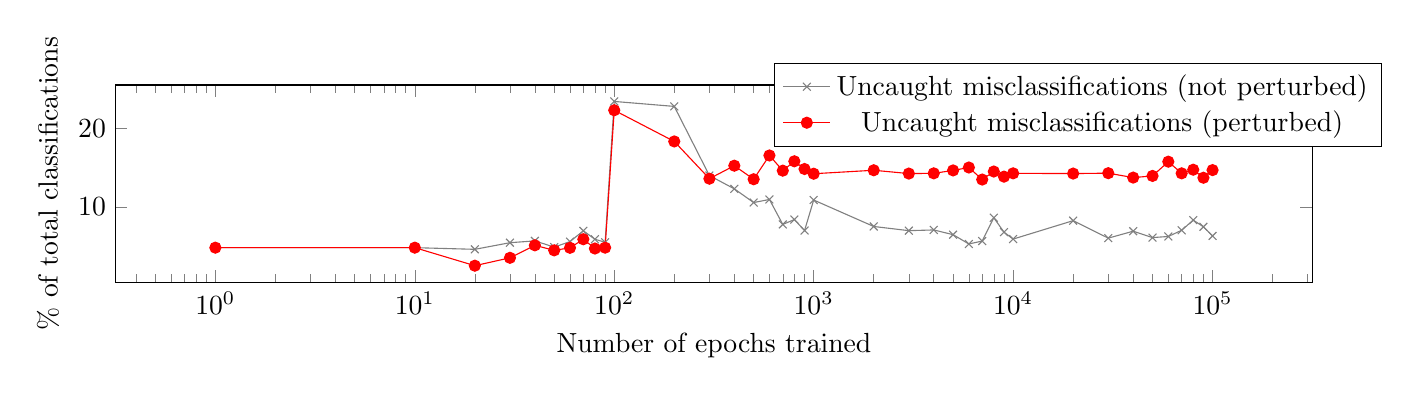
\begin{tikzpicture}
\begin{semilogxaxis}[
xlabel={Number of epochs trained},
ylabel={\% of total classifications},
x=1.1cm,
y=1.0mm, 
legend style={at={(0.55,0.9)},anchor=west}]

\addplot[color=gray,mark=x] coordinates {
	(1, 4.840000)
	(10, 4.840000)
	(20, 4.630000)
	(30, 5.470000)
	(40, 5.700000)
	(50, 4.910000)
	(60, 5.610000)
	(70, 6.980000)
	(80, 5.910000)
	(90, 5.520000)
	(100, 23.410000)
	(200, 22.780001)
	(300, 14.000000)
	(400, 12.310000)
	(500, 10.570000)
	(600, 10.960000)
	(700, 7.790000)
	(800, 8.410000)
	(900, 7.020000)
	(1000, 10.890000)
	(2000, 7.530000)
	(3000, 7.000000)
	(4000, 7.090000)
	(5000, 6.490000)
	(6000, 5.310000)
	(7000, 5.680000)
	(8000, 8.640000)
	(9000, 6.810000)
	(10000, 5.930000)
	(20000, 8.270000)
	(30000, 6.050000)
	(40000, 6.930000)
	(50000, 6.120000)
	(60000, 6.260000)
	(70000, 7.050000)
	(80000, 8.340000)
	(90000, 7.490000)
	(100000, 6.330000)
};

\addplot[color=red,mark=*] coordinates {
	(1, 4.840000)
	(10, 4.840000)
	(20, 2.550000)
	(30, 3.550000)
	(40, 5.140000)
	(50, 4.500000)
	(60, 4.820000)
	(70, 5.910000)
	(80, 4.730000)
	(90, 4.840000)
	(100, 22.290001)
	(200, 18.330000)
	(300, 13.600000)
	(400, 15.250000)
	(500, 13.530000)
	(600, 16.549999)
	(700, 14.620001)
	(800, 15.810000)
	(900, 14.830000)
	(1000, 14.230000)
	(2000, 14.670000)
	(3000, 14.250000)
	(4000, 14.280000)
	(5000, 14.650001)
	(6000, 15.020000)
	(7000, 13.490000)
	(8000, 14.510000)
	(9000, 13.860001)
	(10000, 14.280000)
	(20000, 14.250000)
	(30000, 14.300000)
	(40000, 13.740000)
	(50000, 13.950000)
	(60000, 15.760000)
	(70000, 14.280000)
	(80000, 14.740000)
	(90000, 13.720000)
	(100000, 14.690001)
};

\legend{Uncaught misclassifications (not perturbed), Uncaught misclassifications (perturbed)}
\end{semilogxaxis}%
\end{tikzpicture}%}
	\caption{Line graph showing the number of misclassifications caught by the verifier for the Darkent \ac{MNN} classifier. \label{fig:sign-graphboth}}
\end{figure}

Where input perturbations are concerned, the verifier responded even better and picked up the majority of the total misclassifications.
The verifier caught more misclassifications in untrained \acp{ANN} due to the untrained \acp{ANN} having no confidence about their output.
However, with more trained \acp{ANN} the verifier caught a lower percentage of the total misclassifications due to the \acp{ANN} having a higher confidence that they were correct, even when they were not.

\subsection{An \ac{AV} System Using \acf{MNN2C}}
\ac{MNN2C}, introduced in Section~\ref{sec:mnn2c}, creates time-predictable, modular \acfp{MNN} for C from existing Keras (with Tensorflow) trained \acp{ANN}. 
This compiler makes implementing \acfp{MNN} in C easy and safe.
For the purposes of testing and demonstration, the complex \ac{MNN} used in this chapter, shown in Figure~\ref{fig:mnn}, was trained in Python, using Keras and the exact same images used to train the original, Darknet system.
This \ac{MNN} was then described in the \ac{MNN2C} format, and modular C code was generated to initialise, run and incorporate the \ac{MNN}.
To show the efficacy of \ac{MNN2C}, the generated \ac{MNN} was implemented and tested in an identical system to the original. 
\ac{MNN2C} generates outputs identical to the Keras trained \acp{ANN} with a one hundred-thousandth tolerance, so the output of each individual \ac{SNN} is not being tested here, rather that the system as a whole runs as the original does.
As with the Darknet trained system, the \ac{MNN2C} system was implemented in Esterel and C and run on Ubuntu 16.04, using an 4 core Intel i7-6700HQ processor at 2.6GHz and 4GB of RAM.

\subsubsection{Results of a \ac{MNN2C} generated \ac{AV} system}
The \ac{MNN2C} system was trained in Python using Keras~\cite{chollet2015keras} on Windows 10, using a 4 core Intel i7-6700HQ processor at 2.6GHz and 16GB of RAM.
As a result, Keras was able to use more resources more efficiently than the Darknet library was and, as a result, was able to train \acp{ANN} more efficiently and more quickly than Darknet.
Since these \acp{MNN} were trained in Keras, they did not need to go through same, extensive training to get to a reasonable level of classification accuracy, only needing 100 epochs, as opposed to the 10,000 epochs of training the Darknet \acp{MNN} were trained for.

\begin{figure}[H]
	\centering
	\scalebox{0.9}{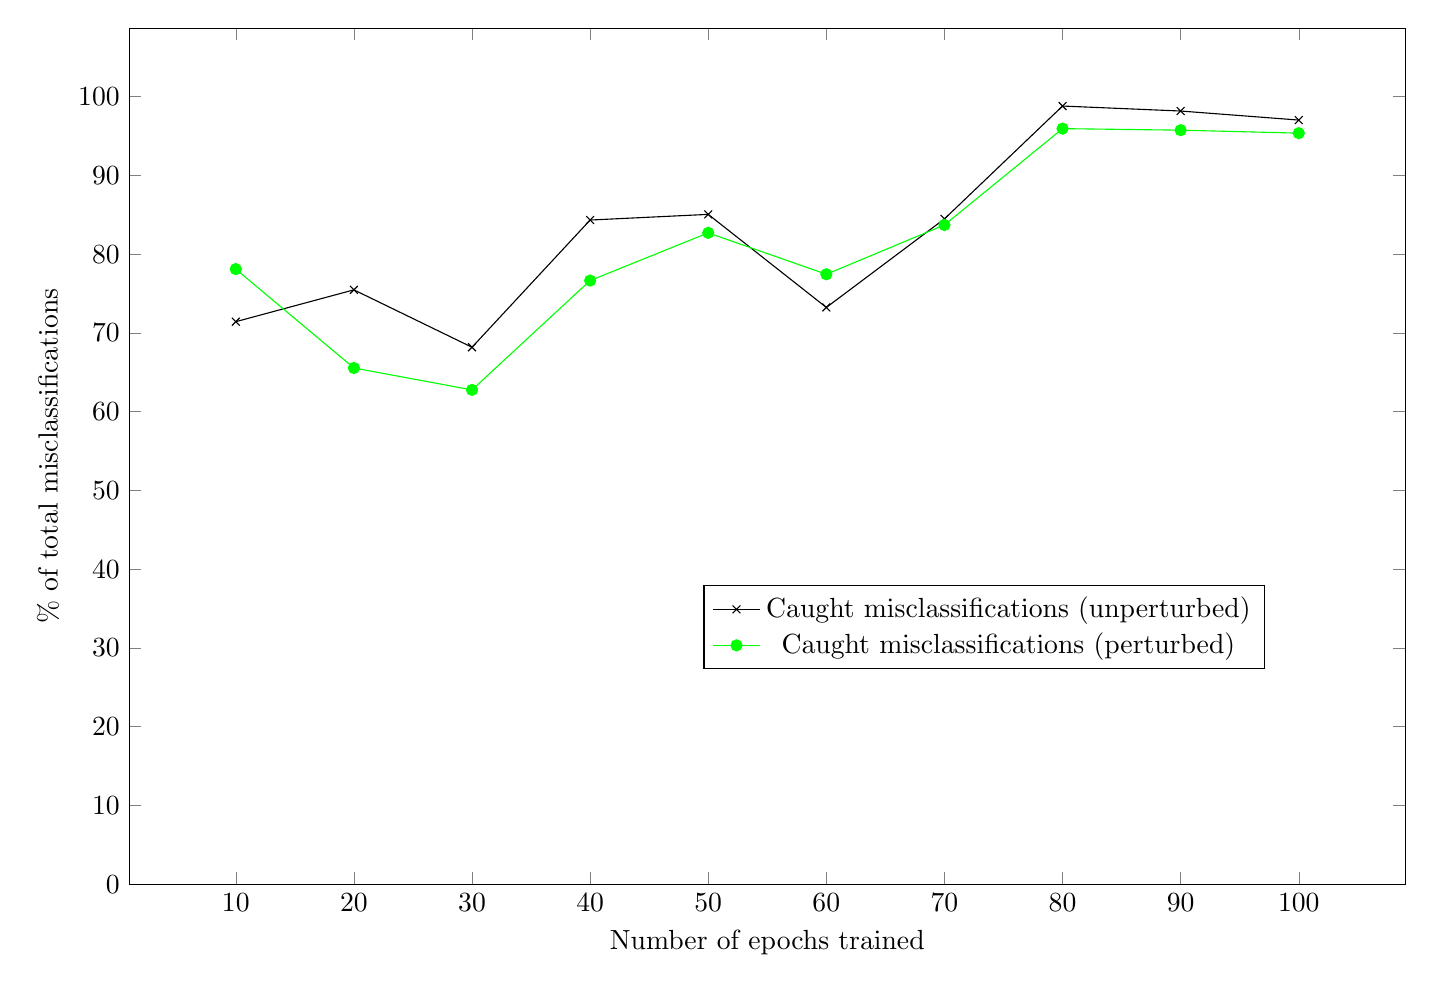
\begin{tikzpicture}
\begin{axis}[
xlabel={Number of epochs trained},
ylabel={\% of total misclassifications},
x=1.5mm, y=1.0mm, 
ymin=0,
legend style={at={(0.45,0.3)},anchor=west}]

\addplot[color=black,mark=x] coordinates {
	(10, 71.428574)
	(20, 75.471695)
	(30, 68.181816)
	(40, 84.337349)
	(50, 85.057472)
	(60, 73.239433)
	(70, 84.482758)
	(80, 98.816566)
	(90, 98.181816)
	(100, 97.033897)
};

\addplot[color=green,mark=*] coordinates {	
	(10, 78.109451)
	(20, 65.550240)
	(30, 62.765957)
	(40, 76.651985)
	(50, 82.710281)
	(60, 77.450981)
	(70, 83.712120)
	(80, 95.945946)
	(90, 95.750000)
	(100, 95.372749)
};

\legend{Caught misclassifications (unperturbed), Caught misclassifications (perturbed)}
\end{axis}%
\end{tikzpicture}%}
	\caption{Line graph showing the number of misclassifications caught by the verifier with \ac{MNN2C} generated \acp{MNN} \label{fig:sign-graphboth-mnn2c}}
\end{figure}

Figure~\ref{fig:sign-graphboth-mnn2c} shows that the verifier stills work efficiently with Keras trained \acp{MNN} compiled to C code.
With the original images, the verifier caught more than 70\% of all misclassifications caught more than 60\% of all misclassifications when the inputs were perturbed.
As the \acp{MNN} are more trained, the number of caught misclassifications increases.
This shows that the system works better with more extensively trained \acp{MNN}.
Unlike the Darknet \acp{MNN}, the verifier was not able to catch 100\% of all the misclassifications for untrained \acp{MNN}.
The \ac{MNN2C} \acp{SNN} used an identical system to the Darknet \acp{SNN}, however they were not trained under identical circumstances, nor were they trained for the same number of epochs.
Thus, by adjusting the system's tolerances to suit the \ac{MNN2C} \acp{SNN}, the system using could likely produce identical results to that of the Darknet \acp{SNN}.
\acp{ANN} trained in Keras are trained slightly differently and, as a result, the confidence of the classifier was different to that of the Darknet classifier.
However, the majority of the misclassifications were still caught, regardless of the number of epochs the classifier was trained for.






















\section{Summary}
This chapter introduces the concept of \acf{RE} in combination with \acf{SANN}.
To facilitate this concept, the previously defined \acfp{MNN} in Chapter 3 are expanded to include non-\ac{ANN} components, such as \acp{RE}.
These are termed \acfp{SNN}.

Sections~\ref{sec:intro} and \ref{sec:related} cover the introduction and related work respectively, providing a case for the use of \ac{RE} in systems with \ac{ANN} in the controllers.

Section~\ref{sec:case} covers the case study used in this chapter.
An \acf{AV} system was chosen to be used as the case study.
\acp{AV} currently have a large influence on the autonomous industry, and being \acfp{CPS}, have relevance in this chapter.

Section~\ref{sec:definitions} covers the definitions for the new formal models introduced in this chapter, most prominently the \acfp{VDTA} used for \ac{RE} and the \acp{SNN} using \ac{RE}.

The last section presents the benchmark results and shows the efficacy of this approach.

\section{Conclusions}

In this work, we have presented an approach for synchronous composition of runtime enforcement with \acfp{ANN} for safety critical systems.
Our \acfp{SNN} demonstrate that policies specifying safe I/O behaviours for \acp{ANN} can be enforced.
This means that their systems can behave in a verifiably safer way.
Our enforcement mechanism, in the three case studies presented, added an average overhead of just 6.035\%.

\subsection{Future Work}

\acp{SANN} supported the concept of meta neural networks, which were synchronous compositions of neural networks. 
In this work, we did not fully examine the enforcement of multiple networks in a meta-neural network (i.e. each network with its own enforcer).
Rather, only our controller networks were \acp{SNN}.
Examining compositions of synchronous neural networks with their enforcers could lead to more capable systems that are still safe. 

\label{sec:conclusion}




\chapter{Conclusions}

This is the conclusion

\section{Future Work}

\begin{comment}
\include{temp}
\end{comment}



% TODO
% Thesis structure sent to Partha
% Flow chart for development




%This is the conclusion

\section{Future Work}

\appendix
\chapter{Appendix}


%\include{Publications}


%%%%%%%%%%%% Last part of thesis indices, bibliography  %%%%%%%%%%%%
\backmatter

%create the bibliography
% \bibliographystyle{siam}
\renewcommand{\bibname}{References}
% \clearpage
\phantomsection
\addcontentsline{toc}{chapter}{\bibname}
\bibliographystyle{IEEEtranS}
\bibliography{references}


\end{document}

